\documentclass{ximera}  


%\usepackage{todonotes}
%\usepackage{mathtools} %% Required for wide table Curl and Greens
%\usepackage{cuted} %% Required for wide table Curl and Greens
\newcommand{\todo}{}

\usepackage{esint} % for \oiint
\ifxake%%https://math.meta.stackexchange.com/questions/9973/how-do-you-render-a-closed-surface-double-integral
\renewcommand{\oiint}{{\large\bigcirc}\kern-1.56em\iint}
\fi


\graphicspath{
  {./}
  {jpg}
  {ximeraTutorial/}
  {basicPhilosophy/}
  {functionsOfSeveralVariables/}
  {normalVectors/}
  {lagrangeMultipliers/}
  {vectorFields/}
  {greensTheorem/}
  {shapeOfThingsToCome/}
  {dotProducts/}
  {partialDerivativesAndTheGradientVector/}
  {../productAndQuotientRules/exercises/}
  {../motionAndPathsInSpace/exercises/}
  {../normalVectors/exercisesParametricPlots/}
  {../continuityOfFunctionsOfSeveralVariables/exercises/}
  {../partialDerivativesAndTheGradientVector/exercises/}
  {../directionalDerivativeAndChainRule/exercises/}
  {../commonCoordinates/exercisesCylindricalCoordinates/}
  {../commonCoordinates/exercisesSphericalCoordinates/}
  {../greensTheorem/exercisesCurlAndLineIntegrals/}
  {../greensTheorem/exercisesDivergenceAndLineIntegrals/}
  {../shapeOfThingsToCome/exercisesDivergenceTheorem/}
  {../greensTheorem/}
  {../shapeOfThingsToCome/}
  {../separableDifferentialEquations/exercises/}
  {vectorFields/}
}

\newcommand{\mooculus}{\textsf{\textbf{MOOC}\textnormal{\textsf{ULUS}}}}

\usepackage{tkz-euclide}\usepackage{tikz}
\usepackage{tikz-cd}
\usetikzlibrary{arrows}
\tikzset{>=stealth,commutative diagrams/.cd,
  arrow style=tikz,diagrams={>=stealth}} %% cool arrow head
\tikzset{shorten <>/.style={ shorten >=#1, shorten <=#1 } } %% allows shorter vectors

\usetikzlibrary{backgrounds} %% for boxes around graphs
\usetikzlibrary{shapes,positioning}  %% Clouds and stars
\usetikzlibrary{matrix} %% for matrix
\usepgfplotslibrary{polar} %% for polar plots
\usepgfplotslibrary{fillbetween} %% to shade area between curves in TikZ
\usetkzobj{all}
\usepackage[makeroom]{cancel} %% for strike outs
%\usepackage{mathtools} %% for pretty underbrace % Breaks Ximera
%\usepackage{multicol}
\usepackage{pgffor} %% required for integral for loops



%% http://tex.stackexchange.com/questions/66490/drawing-a-tikz-arc-specifying-the-center
%% Draws beach ball
\tikzset{pics/carc/.style args={#1:#2:#3}{code={\draw[pic actions] (#1:#3) arc(#1:#2:#3);}}}



\usepackage{array}
\setlength{\extrarowheight}{+.1cm}
\newdimen\digitwidth
\settowidth\digitwidth{9}
\def\divrule#1#2{
\noalign{\moveright#1\digitwidth
\vbox{\hrule width#2\digitwidth}}}





\newcommand{\RR}{\mathbb R}
\newcommand{\R}{\mathbb R}
\newcommand{\N}{\mathbb N}
\newcommand{\Z}{\mathbb Z}

\newcommand{\sagemath}{\textsf{SageMath}}


%\renewcommand{\d}{\,d\!}
\renewcommand{\d}{\mathop{}\!d}
\newcommand{\dd}[2][]{\frac{\d #1}{\d #2}}
\newcommand{\pp}[2][]{\frac{\partial #1}{\partial #2}}
\renewcommand{\l}{\ell}
\newcommand{\ddx}{\frac{d}{\d x}}

\newcommand{\zeroOverZero}{\ensuremath{\boldsymbol{\tfrac{0}{0}}}}
\newcommand{\inftyOverInfty}{\ensuremath{\boldsymbol{\tfrac{\infty}{\infty}}}}
\newcommand{\zeroOverInfty}{\ensuremath{\boldsymbol{\tfrac{0}{\infty}}}}
\newcommand{\zeroTimesInfty}{\ensuremath{\small\boldsymbol{0\cdot \infty}}}
\newcommand{\inftyMinusInfty}{\ensuremath{\small\boldsymbol{\infty - \infty}}}
\newcommand{\oneToInfty}{\ensuremath{\boldsymbol{1^\infty}}}
\newcommand{\zeroToZero}{\ensuremath{\boldsymbol{0^0}}}
\newcommand{\inftyToZero}{\ensuremath{\boldsymbol{\infty^0}}}



\newcommand{\numOverZero}{\ensuremath{\boldsymbol{\tfrac{\#}{0}}}}
\newcommand{\dfn}{\textbf}
%\newcommand{\unit}{\,\mathrm}
\newcommand{\unit}{\mathop{}\!\mathrm}
\newcommand{\eval}[1]{\bigg[ #1 \bigg]}
\newcommand{\seq}[1]{\left( #1 \right)}
\renewcommand{\epsilon}{\varepsilon}
\renewcommand{\phi}{\varphi}


\renewcommand{\iff}{\Leftrightarrow}

\DeclareMathOperator{\arccot}{arccot}
\DeclareMathOperator{\arcsec}{arcsec}
\DeclareMathOperator{\arccsc}{arccsc}
\DeclareMathOperator{\si}{Si}
\DeclareMathOperator{\scal}{scal}
\DeclareMathOperator{\sign}{sign}


%% \newcommand{\tightoverset}[2]{% for arrow vec
%%   \mathop{#2}\limits^{\vbox to -.5ex{\kern-0.75ex\hbox{$#1$}\vss}}}
\newcommand{\arrowvec}[1]{{\overset{\rightharpoonup}{#1}}}
%\renewcommand{\vec}[1]{\arrowvec{\mathbf{#1}}}
\renewcommand{\vec}[1]{{\overset{\boldsymbol{\rightharpoonup}}{\mathbf{#1}}}\hspace{0in}}

\newcommand{\point}[1]{\left(#1\right)} %this allows \vector{ to be changed to \vector{ with a quick find and replace
\newcommand{\pt}[1]{\mathbf{#1}} %this allows \vec{ to be changed to \vec{ with a quick find and replace
\newcommand{\Lim}[2]{\lim_{\point{#1} \to \point{#2}}} %Bart, I changed this to point since I want to use it.  It runs through both of the exercise and exerciseE files in limits section, which is why it was in each document to start with.

\DeclareMathOperator{\proj}{\mathbf{proj}}
\newcommand{\veci}{{\boldsymbol{\hat{\imath}}}}
\newcommand{\vecj}{{\boldsymbol{\hat{\jmath}}}}
\newcommand{\veck}{{\boldsymbol{\hat{k}}}}
\newcommand{\vecl}{\vec{\boldsymbol{\l}}}
\newcommand{\uvec}[1]{\mathbf{\hat{#1}}}
\newcommand{\utan}{\mathbf{\hat{t}}}
\newcommand{\unormal}{\mathbf{\hat{n}}}
\newcommand{\ubinormal}{\mathbf{\hat{b}}}

\newcommand{\dotp}{\bullet}
\newcommand{\cross}{\boldsymbol\times}
\newcommand{\grad}{\boldsymbol\nabla}
\newcommand{\divergence}{\grad\dotp}
\newcommand{\curl}{\grad\cross}
%\DeclareMathOperator{\divergence}{divergence}
%\DeclareMathOperator{\curl}[1]{\grad\cross #1}
\newcommand{\lto}{\mathop{\longrightarrow\,}\limits}

\renewcommand{\bar}{\overline}

\colorlet{textColor}{black}
\colorlet{background}{white}
\colorlet{penColor}{blue!50!black} % Color of a curve in a plot
\colorlet{penColor2}{red!50!black}% Color of a curve in a plot
\colorlet{penColor3}{red!50!blue} % Color of a curve in a plot
\colorlet{penColor4}{green!50!black} % Color of a curve in a plot
\colorlet{penColor5}{orange!80!black} % Color of a curve in a plot
\colorlet{penColor6}{yellow!70!black} % Color of a curve in a plot
\colorlet{fill1}{penColor!20} % Color of fill in a plot
\colorlet{fill2}{penColor2!20} % Color of fill in a plot
\colorlet{fillp}{fill1} % Color of positive area
\colorlet{filln}{penColor2!20} % Color of negative area
\colorlet{fill3}{penColor3!20} % Fill
\colorlet{fill4}{penColor4!20} % Fill
\colorlet{fill5}{penColor5!20} % Fill
\colorlet{gridColor}{gray!50} % Color of grid in a plot

\newcommand{\surfaceColor}{violet}
\newcommand{\surfaceColorTwo}{redyellow}
\newcommand{\sliceColor}{greenyellow}




\pgfmathdeclarefunction{gauss}{2}{% gives gaussian
  \pgfmathparse{1/(#2*sqrt(2*pi))*exp(-((x-#1)^2)/(2*#2^2))}%
}


%%%%%%%%%%%%%
%% Vectors
%%%%%%%%%%%%%

%% Simple horiz vectors
\renewcommand{\vector}[1]{\left\langle #1\right\rangle}


%% %% Complex Horiz Vectors with angle brackets
%% \makeatletter
%% \renewcommand{\vector}[2][ , ]{\left\langle%
%%   \def\nextitem{\def\nextitem{#1}}%
%%   \@for \el:=#2\do{\nextitem\el}\right\rangle%
%% }
%% \makeatother

%% %% Vertical Vectors
%% \def\vector#1{\begin{bmatrix}\vecListA#1,,\end{bmatrix}}
%% \def\vecListA#1,{\if,#1,\else #1\cr \expandafter \vecListA \fi}

%%%%%%%%%%%%%
%% End of vectors
%%%%%%%%%%%%%

%\newcommand{\fullwidth}{}
%\newcommand{\normalwidth}{}



%% makes a snazzy t-chart for evaluating functions
%\newenvironment{tchart}{\rowcolors{2}{}{background!90!textColor}\array}{\endarray}

%%This is to help with formatting on future title pages.
\newenvironment{sectionOutcomes}{}{}



%% Flowchart stuff
%\tikzstyle{startstop} = [rectangle, rounded corners, minimum width=3cm, minimum height=1cm,text centered, draw=black]
%\tikzstyle{question} = [rectangle, minimum width=3cm, minimum height=1cm, text centered, draw=black]
%\tikzstyle{decision} = [trapezium, trapezium left angle=70, trapezium right angle=110, minimum width=3cm, minimum height=1cm, text centered, draw=black]
%\tikzstyle{question} = [rectangle, rounded corners, minimum width=3cm, minimum height=1cm,text centered, draw=black]
%\tikzstyle{process} = [rectangle, minimum width=3cm, minimum height=1cm, text centered, draw=black]
%\tikzstyle{decision} = [trapezium, trapezium left angle=70, trapezium right angle=110, minimum width=3cm, minimum height=1cm, text centered, draw=black]




 
\title{Electrostatic Force} 
\author{Milica Markovic} 
\outcome{Electrostatic force.}
\begin{document}  
\begin{abstract}  

\end{abstract}  
\maketitle    



\section{Electic Charges}
 Electric charges observed in nature are multiples of a charge of an electron $e=-1.6 10^{-19}$\,C. JJ Thomson discovered the electron in his cathode ray tube experiments in  1897. R. Millikan measured the mass to charge ratio of the electron in 1909 through his oil-drop experiment.  In 1960, J. G. King proved experimentally that one proton carries a positive charge of $e=1.6 10^{-19}$\,C. 



\section{Electrostatic Force}

The electrostatic force acts between electric charges in the following way:

\begin{itemize}
\item two positive charges repel each other.
\item two negative charges repel each other.
\item a positive and a negative charge attract each other.
\item the force between two charges decreases inversely proportional to the square of the distance.
\item the force acts along the line that connects the charges.
\item in nature, positive and negative charges are balanced, and the net result is electrical neutrality! Balance is formed by tight fine mixtures of positive and negative charges.
\end{itemize}
 
 A demonstration of the electric force  by 
 the MIT professor emeritus Walter Lewin.
 
 \begin{center}
 \youtube{x1-SibwIPM4?t=2550}
 \end{center}
 
 
 \section{Coulomb's Law}

What we described is exactly the electrostatic force. All matter is a mixture of positive protons and negative electrons in a perfect balance. Coulomb described the strength and direction of the electrostatic force through his torsion-balance experiment in 1785.  We can represent this electrostatic force visually. Figure \ref{twostaticch} shows a stationary charge $+q_1$, repelling charge $+q_2$ with a force $F_{2}$. The figure shows the unit vector $\hat{r}_{21}$, and the distance vector $\vec{R}_{21}=r_{21} \hat{r}_{21}$, where $r_{21}=|\vec{R}_{21}|$ is the distance between the two point charges. The equation that describes the electrostatic (Coulomb) force $\vec{F}_2$ is given in Equation \ref{EqCoulombslaw}.


\begin{eqnarray}
\vec{F_2}=\frac{q_1 q_2}{4 \pi \epsilon_0 r_{21}^2} \hat{r}_{21} \label{EqCoulombslaw}
\end{eqnarray}

In the above equation, $\epsilon_0=8.81\, 10^{-12}$\,F/m is the electrical permittivity of air, $r_{21}$ is the distance between charges, vector $\hat{r}_{21}$ is a unit vector oriented from charge 1 to charge 2. The unit vector is on the line that connects charges 1 and 2, and therefore the electrostatic force is also on the line that connects the two charges. The force will either point in the direction of the unit vector if the force is repulsive (charges have the same sign), or in the opposite direction when the force is attractive (charges have the opposite sign). Note that we need at least two charges to find the electrostatic force.


\begin{figure}[htbp]
\begin{center}
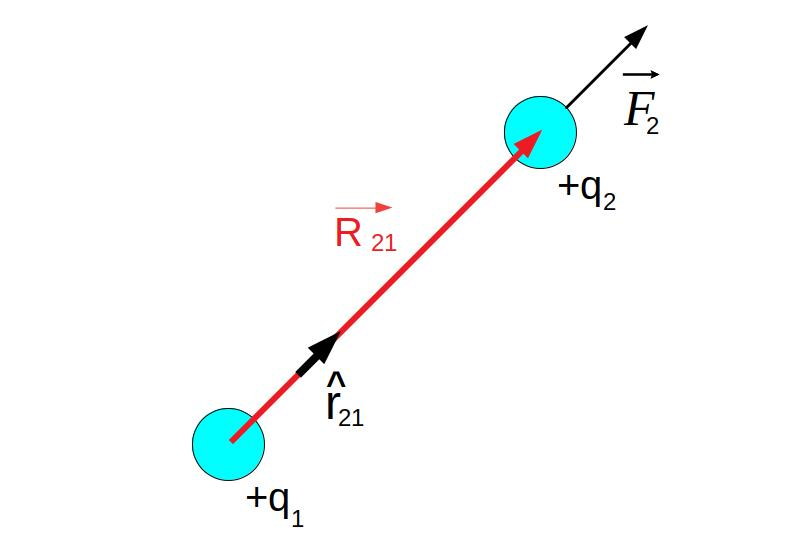
\includegraphics[scale=0.5]{../jpg/Two_Static_ChargesV1.jpg}
\end{center}
\caption{Vector representation of Coulomb's force between two static charges.}
\label{twostaticch}
\end{figure}




If the total net charge of an object is $q$, and if that object has $n_e$ electrons and $n_p$ protons, then the total charge is $q=n_p e-n_e e$. 



\begin{example} 
Two positive unit charges $q_1=1$\,nC and $q_2=1$\,nC are fixed in air in Cartesian coordinate system at points $A(x_1,y_1,z_1)$ and $B(x_2,y_2,z_2)$, see Figure \ref{FigTwoCharges}. Find the electric force that charge at point A exerts on charge at point B, and the force that charge at point B exerts on charge at point A. How would your answer change if one charge becomes negative? 



\begin{figure}[htbp]
\begin{center}
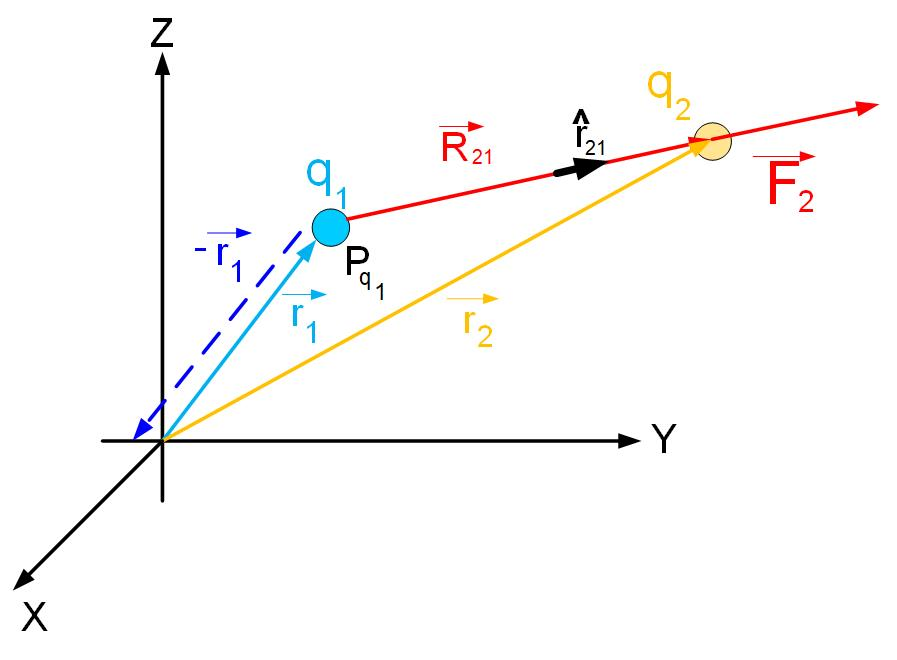
\includegraphics[scale=0.5]{../jpg/twochargecartcoordFORCE.jpg}
\end{center}
\caption{Electric Field due to a unit charge in Rectangular coordinate system.}
\label{FigTwoCharges}
\end{figure}

\begin{explanation}

The electrostatic force $F_2$ on charge $q_2$ is given by 




\begin{eqnarray}
\vec{F_2}=\frac{q_1 q_2}{4 \pi \epsilon_0 r_{21}^2} \hat{r}_{21}
\end{eqnarray}

 To find the force, we have to calculate

\begin{enumerate} 
\item The magnitude of the force $|\vec{F_2}|=\frac{q_1 q_2}{4 \pi \epsilon_0 r_{21}^2}$. To find the magnitude, we need to find the distance between the two charges $r_{21}$. To find the distance, we need to find the distance vector $\vec{R}_{21}$. 
\item To find the unit vector, we need to find the distance vector first. $\hat{r}_{21}=\frac{\vec{R}_{21}}{r_{21}}$.
\end{enumerate}

The distance vector is a particular type of vector that starts at one point in the coordinate system and ends at another point. To find the distance vector $\vec{R}_{21}$, we first have to know the position of charge $q_1$, where the distance vector starts, and the position of charge $q_2$ where the distance vector ends. In this problem, the location of two charges is given by two points in the coordinate system A and B.  

The next step is finding the position vector $r_1$ of point A, and the position vector $r_2$ of point B. Position vectors are special vectors that start in the coordinate system origin and point to various points in the coordinate system. Charge $q_1$ is at point $A(x_1,y_1,z_1)$, therefore the position vector $\vec{r_1}$ of this point is  shown in Equation \ref{Eqposvec1}.


\begin{eqnarray}
\vec{r_1}=x_1 \vec{x} + y_1 \vec{y} +z_1 \vec{z} \label{Eqposvec1}
\end{eqnarray}

The position vector of charge $q_2$ is 

\begin{eqnarray}
\vec{r_2}=x_2\vec{x} + y_2 \vec{y} +z_2 \vec{z}
\end{eqnarray}

The two vectors mark the beginning and the end of the distance vector $\vec{R}_{21}$  between charges $q_1$ and $q_2$. The vector  $\vec{R}_{21}$ is the sum of vectors $-\vec{r_1}$ and $\vec{r_2}$. 



\begin{eqnarray}
\vec{R}_{21}=\vec{r_2} + (-\vec{r_1})
\end{eqnarray}

When we substitute position vectors $r_1$ and $r_2$:

\begin{eqnarray}
\vec{R}_{21}= (x_2 - x_1) \vec{x} +(y_2 - y_1) \vec{y} +(z_2 - z_1) \vec{z}
\end{eqnarray}

The magnitude of vector $\vec{R}_{21}$ is


\begin{eqnarray}
|\vec{R}_{21}|= \sqrt{(x_2 - x_1)^2 +(y_2 - y_1)^2 +(z_2 - z_1)^2}
\end{eqnarray}

Unit vector in the direction of vector $\vec{R}_{21}$ is:


\begin{eqnarray}
\hat{r}_{21}= \frac{\vec{R}_{21}}{|\vec{R}_{21}|} \\
\hat{r}_{21}=\frac{\vec{R}_{21}}{\sqrt{(x_2 - x_1)^2 +(y_2 - y_1)^2 +(z_2 - z_1)^2}}
\end{eqnarray}

Substituting expressions for $\hat{r}_{21}$, and $|\vec{R}_{21}|$ in equation for the electrostatic force 

\begin{eqnarray}
\vec{F_2}=\frac{q_1 q_2}{4 \pi \epsilon_{0} {r_a}^2} \hat{r_a}
\end{eqnarray}

 

 
We get


\begin{eqnarray}
\vec{F_2}=\frac{q_1 q_2}{4 \pi \epsilon_{0} {\sqrt{(x_2 - x_1)^2 +(y_2 - y_1)^2 +(z_2 - z_1)^2}
}^3} \vec{R}_{21} \label{eqonecharge}
\end{eqnarray}







\end{explanation}


\end{example}




\subsubsection{What if the charge is in an insulator (aka dielectric) other than air?} 

If the charge is within a dielectric material, then we need to account for that by changing this $\epsilon_0$ somehow. If we place the charge inside a dielectric material, what do you think will happen with the atoms in the material? The atoms will get distorted and polarized. Such a polarized atom we call an electric dipole. The distortion process is called polarization. Because the material polarizes, the electric field around this point charge is different than if there was no material. To compensate for this new polarization, we multiply the dielectric permittivity of free space $\epsilon_0$ with a unitless quantity of $\epsilon_r$.  $\epsilon_r$ is called a relative dielectric constant. $\epsilon_r$ values for different materials can found on the internet. Some examples of dielectric constants are $\epsilon_r$: air $\epsilon_r$=1,  Teflon $\epsilon_r$=2.2, glass $\epsilon_r$=4.4, Silicon $\epsilon_r$= 11, GaAs $\epsilon_r$=12, distilled water $\epsilon_r$= 80.  Equation \ref{EqCoulombslaw3} is the definition of the electrostatic force between two charges. Sometimes, the product of $\epsilon_0 \epsilon_r$ is written as $\epsilon$.

\begin{eqnarray}
\vec{F_e}=\frac{q_1 q_2}{4 \pi \epsilon_0 \epsilon_r r^2} \hat{R_{12}} \label{EqCoulombslaw3} \\
\epsilon = \epsilon_0 \epsilon_r
\end{eqnarray}



\subsection{Principle of Superposition}

If we have four charges, the total force from three charges to one charge is equal to the vector sum of the forces due to individual charges, see Figure \ref{superpositionforce}.  The field at



\begin{figure}[htbp]
\begin{center}
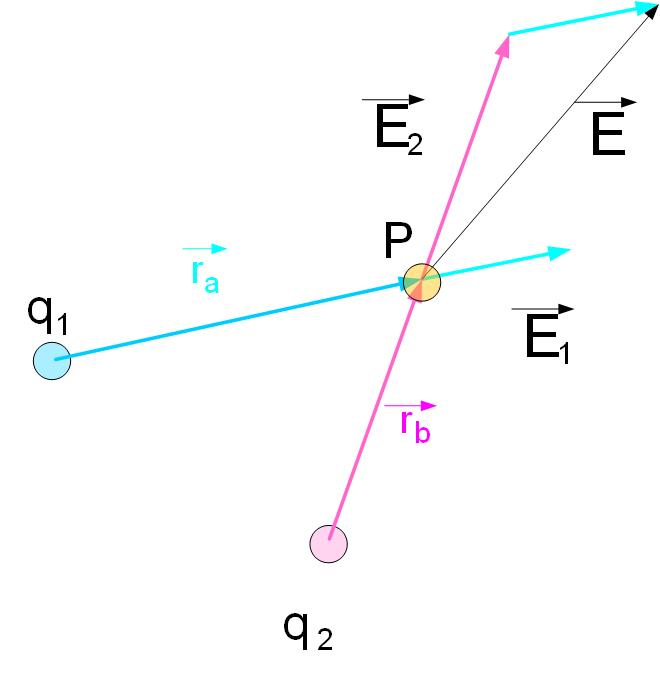
\includegraphics[scale=0.5]{../jpg/superpositionFORCE.jpg}
\end{center}
\caption{Electric Field due to two charges.}
\label{UnitCh}
\end{figure}

The fields or charges $q_1$ and $q_2$ are:

\begin{eqnarray}
\vec{F_1}=\frac{q_1}{4 \pi \epsilon_{0} {r_a}^2} \hat{r_a} \label{field}\\
\vec{F_2}=\frac{q_1}{4 \pi \epsilon_{0} {r_b}^2} \hat{r_b}
\end{eqnarray}

Where $\hat{r_a}$ and $\hat{r_b}$ are unit vectors in the direction of $r_a$ and $r_b$. The total field due to both charges is


\begin{eqnarray}
\vec{F}=\vec{F_1} + \vec{F_2} 
\end{eqnarray}




If charge $q_3$, is at a point $C(x_3,y_3,z_3)$ as shown in Figure \ref{threecharges} the force on charge $q_2$  becomes

\begin{eqnarray}
\vec{F}= \frac{q_1 q_2}{4 \pi \epsilon_{0} {\sqrt{(x_2 - x_1)^2 +(y_2 - y_1)^2 +  (z_2 - z_1)^2}^3}} \vec{R}_{21} + \\ \nonumber
 \frac{q_2 q_3}{4 \pi \epsilon_{0} {\sqrt{(x_2 - x_3)^2 +(y_2 - y_3)^2 +(z_2 - z_3)^2}
}^3} \vec{R}_{23} 
\end{eqnarray}



\begin{figure}[htbp]
\begin{center}
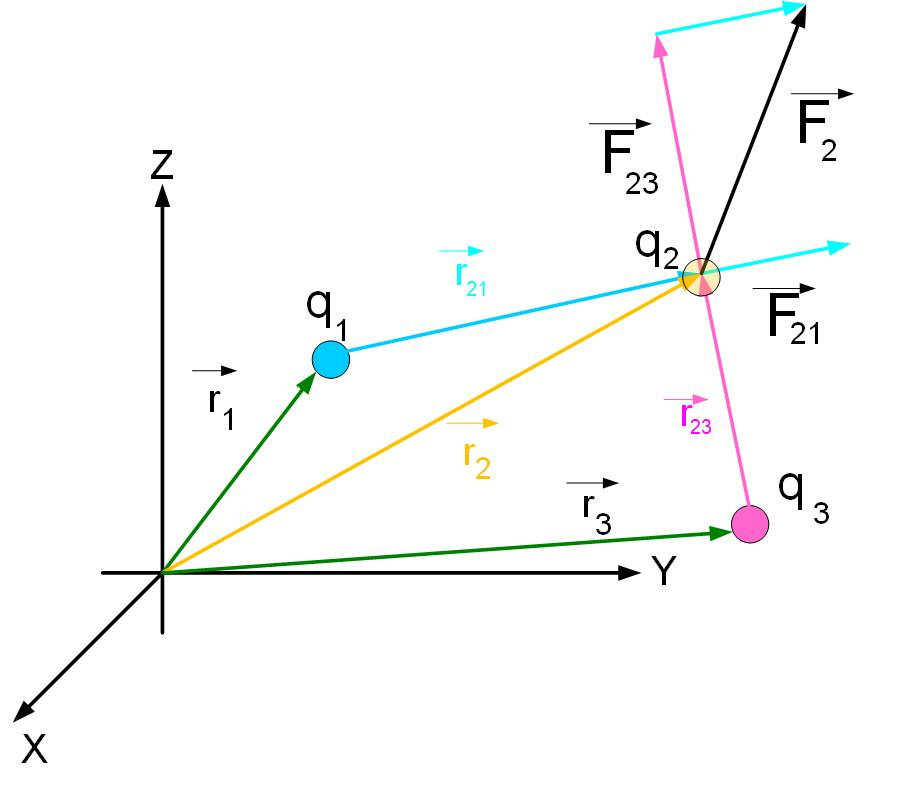
\includegraphics[scale=0.5]{../jpg/twochargescartcoordFORCE.jpg}
\end{center}
\caption{Electric field due to two charges in  Rectangular coordinate system.}
\label{singlecharge}
\end{figure}



\begin{problem}

Three positive charges, each $q=100\mu C$ are placed at A(0,0), B(8,0) and C(4,4). Calculate the magnitude and direction of total force exerted on B, due to charges A and C. Check your result with the calculator below. Explore with the calculator below how would the direction of net force on B change if the charges A and C become negative. 
\begin{center}
\geogebra{xqytpecf}{1200}{800}
\end{center}

\end{problem}


\begin{question}  
  Four negative charges Q are distributed at (-1,0), (1,0), (0,1) and (0, -1). If we place the fifth charge Q at the origin (0,0), what will be the total force on this charge regardless of it's polarity?  
  \begin{multipleChoice}  
    \choice[correct]{$0$}  
    \choice{"Not enough information"}  
    \choice{$\frac{4 Q^2}{4 \pi \epsilon_0}$}  
    \choice{$\frac{-4 Q^2}{4 \pi \epsilon_0}$}  
  \end{multipleChoice}  
\end{question}



\end{document}